\clearpage

\section{Implementing an OAuth client}
\label{sec:implementation}
This chapter describes a practical implementation for an OAuth 2.0 client using an authorization server provided by a third party.
The central design choices are described in addition to their effect on the security of the system.
The OAuth client consists of a minimal frontend application that interacts with an API backend which handles all communication with the authorization server.
The backend supports using multiple authorization servers simultaneously, with the example implementing authorization using Google and Microsoft accounts.
The focus of the chapter lies on the authorization code flow, as the process of retrieving an access token is the most critical part of an OAuth system.
It should also be possible to implement the authorization code flow in a similar way as in the example for a wide variety of different applications.
The chapter briefly describes token introspection and token refreshing, but as their implementation will vary greatly between different applications, they are not described in detail.
The complete source code for the client can be found on GitHub \citep{noauthor_backjonasoauth-client_nodate}.
 

\subsection{Application structure}

When implementing a modern web application, developers are left with a number of choices.
As described in section \ref{sec:background-structure}, the utilization of JavaScript allows developers to implement complete applications that are fully contained on the end user's machine.
When implementing an OAuth client, it is possible to contain all logic on the client machine.
This does however negatively affect the overall security of the system.
Single-page applications (SPAs), where all logic is contained in the browser, are considered public OAuth clients, as a user can access and study every part of the system.
In such clients, the authorization code flow can only be partially implemented, as it relies on the client proving its identity using a client secret.
As the client is completely stored in the user's machine, a malicious user can simply analyze the application and retrieve the secret value.
As the benefits provided by the authorization code flow are not fully realized in public clients, they often utilize the implicit grant instead, which is inherently less secure than the authorization code flow.

Due to these limitations of pure SPAs, the example implementation splits the OAuth client into a frontend and a separate API backend.
The user interacts with the frontend which in turn interacts with the API.
The API is responsible for all communication with the authorization server, allowing the client to securely store client secrets.
The separate API also makes it possible to more securely store access tokens and other secrets belonging to the end user.
These storage options are described in detail in sections \ref{sec:implementation-storage} - \ref{sec:pkce}.

\subsubsection{Obtaining an access token}
\label{sec:implementation:access-token}

The OAuth client implements the authorization code grant to authenticate users.
As the client is separated into two parts, some additional steps are required compared to a minimal authorization code grant.
The network traffic of the authorization flow is shown in figure \ref{client_auth_requests}.
Each step in the authorization flow is detailed below, with code snippets describing how they are implemented.

\begin{figure}[b]
	\centering
    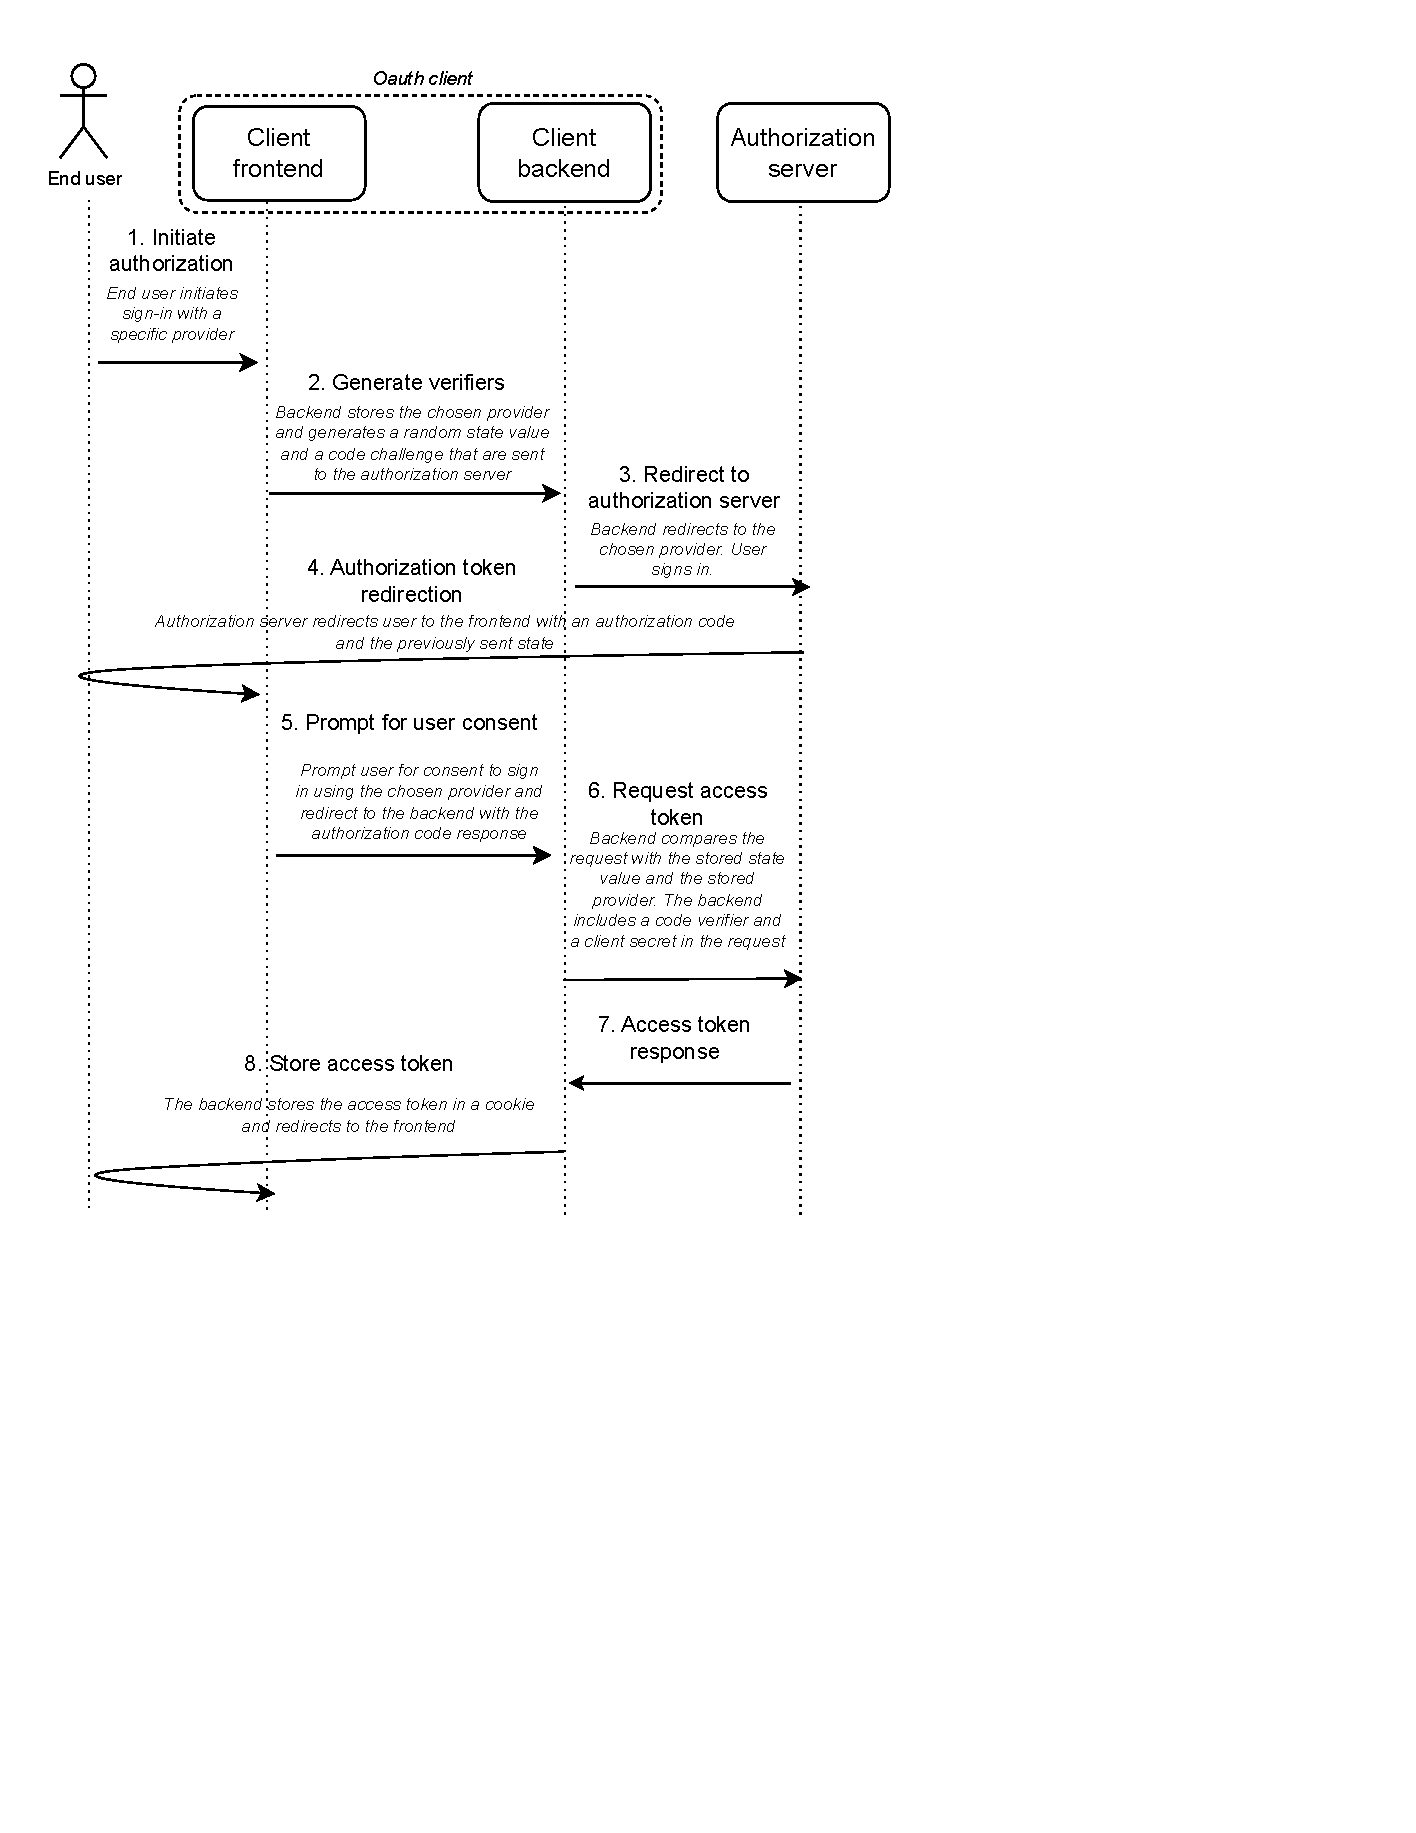
\includegraphics[height=185mm]{assets/client_request_flow.drawio.pdf}
	\caption{Network traffic of the OAuth clients authentication flow}
	\label{client_auth_requests}
\end{figure}

\clearpage
\begin{enumerate}
    \item \textbf{Initiate authorization} \\
    The user begins the sign-in process by clicking on a button to sign in with a specific provider.
\begin{lstlisting}[style=ES6, caption={Login button}]
const LoginButton = ({ provider }: { provider: string }) => {
  return (
    <button
      onClick={() =>
        (window.location.href = `${API_URL}/oauth/login/${provider}`)
      }
    >
      Login with {provider}
    </button>
  )
}
\end{lstlisting}
%\end{enumerate}

%\begin{enumerate}
%  \setcounter{enumi}{1}
    \item \textbf{Generate verifiers} \\
    The user is redirected to the client backend to a route belonging to the chosen provider.
    The backend server generates two random 32 byte strings, with one string used as a state value and the other string used as a code verifier.
    A code challenge is created based on the code verifier to be used by PKCE, described in more detail in section \ref{sec:pkce}.
    The backend stores the code verifier, the state value as well as the chosen provider as cookies in the user's browser. \\
    The code challenge is generated with the following function:
    \begin{lstlisting}[style=ES6, caption={Code challenge generation}]
export const generateCodeChallenge = (codeVerifier: string) => {
  return base64url(crypto.createHash('sha256').update(codeVerifier).digest())
}
\end{lstlisting}
    \item \textbf{Redirect to authorization server} \\
    The user is redirected to the chosen authorization server.
    The state and code challenge generated in the previous step are included as query parameters, in addition to a \textit{redirect URI}, to which the authorization server will redirect the user after successfully authenticating.
    A client id provided by the authorization server is also included, as well as the \textit{access\_type} which indicates whether a refresh token should be included. \\
    The URL to the authorization server is constructed with the following function:
    
\begin{lstlisting}[style=ES6, caption={Constructing the authorization server URL}]
export const getAuthServer = async (
  state: string,
  codeChallenge: string,
  provider: string
) => {
  const endpoint = await getEndpoint('authorization_endpoint', provider)
  const oauthCredentials = config.providers[provider]
  if (endpoint === undefined || oauthCredentials === undefined) {
    return undefined
  }

  // Refresh token should be requested as part of the scope  
  // for Microsoft, while it is requested from other
  // providers with access_type='offline'
  const scope = provider === 'microsoft' ? 'offline_access openid' : 'openid'

  return (
    endpoint +
    '?response_type=code' +
    `&client_id=${oauthCredentials.clientId}` +
    `&scope=${scope}` +
    `&redirect_uri=${config.redirectUri}/${provider}` +
    '&access_type=offline' +
    `&state=${state}` +
    `&code_challenge=${codeChallenge}` +
    '&code_challenge_method=S256'
  )
}
\end{lstlisting}

    The complete login route is implemented as follows, where \textit{oauthRouter} is an express router \citep{noauthor_express_nodate}:
\begin{lstlisting}[style=ES6, caption={Login route}]
oauthRouter.get('/login/:provider', async (req: Request, res: Response) => {
  const { provider } = req.params
  const state = randomBytes(32).toString('hex')
  const codeVerifier = base64url(randomBytes(32))
  const codeChallenge = generateCodeChallenge(codeVerifier)

  const authServer = await getAuthServer(state, codeChallenge, provider)
  if (authServer === undefined) {
    return res.sendStatus(500)
  }

  res.cookie('state', state, {
    httpOnly: true,
    secure: true,
    sameSite: 'lax',
    signed: true,
    maxAge: 60 * 1000,
  })

  res.cookie('code_verifier', codeVerifier, {
    httpOnly: true,
    secure: true,
    sameSite: 'lax',
    signed: true,
    maxAge: 60 * 1000,
  })

  res.cookie('provider', provider, {
    httpOnly: true,
    secure: true,
    sameSite: 'lax',
    signed: true,
  })

  res.redirect(authServer)
})
\end{lstlisting}

    \item \textbf{Authorization token redirection} \\
    After authenticating the user, the authorization server redirects the user to the client frontend, which was defined as a \textit{redirect URI}.
    The redirect includes an authorization code as well as the previously defined state parameter.
    \item \textbf{Prompt for user consent} \\
    The client asks the user to confirm that they wish to authenticate using the chosen provider.
    This step is not part of the authorization code grant flow, but is included as an additional guard against CSRF.
    The additional protection is needed, as a user could be tricked to initiate the authorization process by clicking a malicious link.
    As the user is redirected to this page by the \textit{redirect URI} parameter set in step 3, a user authenticating using a specific provider can only be redirected to one confirmation page, as long as the authorization server is not incorrectly configured.
    This protection is provided by the fact that authorization servers require setting all allowed redirect URIs, and as only one URI is needed for the flow, redirection can be limited to one allowed path per provider.
    After consenting to the authorization, the user is redirected to the backend, forwarding the authorization code and state parameter the authorization server sent. \\
    The consent page is implemented as the following React \citep{noauthor_react_nodate} component.

\begin{lstlisting}[style=ES6, caption={User consent page}]
import { useParams } from 'react-router-dom'

const API_URL = import.meta.env.API_URL

export const OAuthCallbackPage = () => {
  const { provider } = useParams()
  const { searchParams } = new URL(document.location.toString())
  return (
    <>
      <h1>Login confirmation</h1>
      {provider === undefined ? (
        <p>Authentication error</p>
      ) : (
        <>
          <p>Do you wish to continue authenticating using {provider}?</p>
          <button
            onClick={() =>
              (window.location.href = `${API_URL}/oauth/code/${provider}?${searchParams.toString()}`)
            }
          >
            Continue
          </button>
        </>
      )}
    </>
  )
}
\end{lstlisting}

    \item \textbf{Request access token} \\
    The backend fetches the state, code verifier and provider that were stored as cookies in step 2.
    The previously stored state and provider are compared with the values in the current request, and if either value does not match the authorization process is aborted.
    The following steps are taken to validate the request:
    \begin{lstlisting}[style=ES6, caption={Part of the backend code callback route that deals with validating the request}]
oauthRouter.get('/code/:provider', async (req: Request, res: Response) => {
  // Verify that a authorization code was provided
  // and that a code verifier has been stored in the client cookies
  const code = req.query?.code
  const codeVerifier = req.signedCookies?.code_verifier
  if (typeof code !== 'string' || typeof codeVerifier !== 'string') {
    return res.sendStatus(400)
  }

  // Verify that the state sent in the original authorization request matches
  // with the state provided in the callback
  const codeState = req.query?.state
  const cookieState = req.signedCookies['state'] as string | undefined
  if (
    typeof codeState !== 'string' ||
    typeof cookieState !== 'string' ||
    codeState === '' ||
    codeState !== cookieState
  ) {
    return res.sendStatus(403)
  }

  // Verify that the provider of the oauth callback matches with the
  // provider of the original login request
  const previousProvider = req.signedCookies?.provider
  const provider = req.params.provider
  if (
    typeof previousProvider !== 'string' ||
    typeof provider !== 'string' ||
    provider !== previousProvider
  ) {
    return res.sendStatus(403)
  }
  ...
})
\end{lstlisting}

    If all the validation steps pass, an access token is requested from the authorization server based on the authorization code.
    It includes the same client id as in the original authorization request, with an additional client secret.
    The original code verifier and redirect URI are also included. \\
    The access token is requested with the following function:
    \begin{lstlisting}[style=ES6, caption={Function used to request an access token and refresh token}]
export const getToken = async (
  code: string,
  codeVerifier: string,
  provider: string
): Promise<TokenResponse | undefined> => {
  const endpoint = await getEndpoint('token_endpoint', provider)
  const configCredentials = config.providers[provider]
  if (endpoint === undefined || configCredentials === undefined) {
    return undefined
  }

  const client_id = configCredentials.clientId
  const client_secret = configCredentials.clientSecret
  const redirect_uri = `${config.redirectUri}/${provider}`
  const grant_type = 'authorization_code'
  const code_verifier = codeVerifier

  try {
    const authResponse = await fetch(endpoint, {
      method: 'POST',
      body: new URLSearchParams({
        client_id,
        client_secret,
        redirect_uri,
        grant_type,
        code,
        code_verifier,
      }),
      headers: {
        'Content-Type': 'application/x-www-form-urlencoded',
      },
    })
    if (!authResponse.ok) {
      return undefined
    }
    return (await authResponse.json()) as TokenResponse
  } catch (error) {
    console.error(error)
    return undefined
  }
}
\end{lstlisting}
    \item \textbf{Access token response} \\
    The authorization server verifies the code verifier and checks that the redirect URI matches with the URI of the original code request.
    If the checks pass, the server responds with an access token, as well as an optional refresh token and id token, if they were requested in the code request.
    \item \textbf{Store access token} \\
    The backend stores the access token and optional refresh token as cookies and redirects the user to the landing page of the frontend.
    The token storage is described in greater detail in section \ref{sec:implementation-storage}.
    When the user makes a request to the backend in the future, the server will be able to identify the user based on this access token. \\
    The token storage and user redirection is handled as follows:
\begin{lstlisting}[style=ES6, caption={Part of the backend code callback route that deals with storing tokens and redirecting the user to the frontend}]
oauthRouter.get('/code/:provider', async (req: Request, res: Response) => {
  ...
  const token = await getToken(code, codeVerifier, provider)
  if (token !== undefined) {
    res.cookie('access_token', token.access_token, {
      httpOnly: true,
      secure: true,
      sameSite: 'strict',
      signed: true,
      maxAge: token.expires_in * 1000,
    })

    res.cookie('refresh_token', token.refresh_token, {
      httpOnly: true,
      secure: true,
      sameSite: 'strict',
      signed: true,
    })
  }

  res.redirect(config.frontendOrigin)
})
\end{lstlisting}
\end{enumerate}

\subsubsection{Inspecting existing access tokens}

OAuth access tokens are typically opaque, and as such a client can not extract any information from the token itself.
If an OAuth client wants to identify a user and confirm that an access token is valid, it must send an introspection request to the authorization server.
The token introspection flow is described in figure \ref{introspection_client_flow}.
The token introspection relies on an access token and a provider that were stored when obtaining an access token.
Many frontend libraries require explicitly including cookies to send them in any requests.
In our TypeScript example using the fetch() global function \citep{noauthor_fetch_2023}, cookies can be included with the \textit{credentials: 'include'} option.
The backend application must also set the Access-Control-Allow-Credentials header in the response to signal that cookies are used to identify requests.

Based on the type of token, the authorization server can return a differing amount of information, such as user emails and names.
The minimal information that it will return however is a unique \textit{sub} value, which is a unique identifier for the token subject.
When combining this sub value with the token provider, the OAuth client can identify a user, allowing the client application to serve personalized content.

\begin{figure}[b]
	\centering
    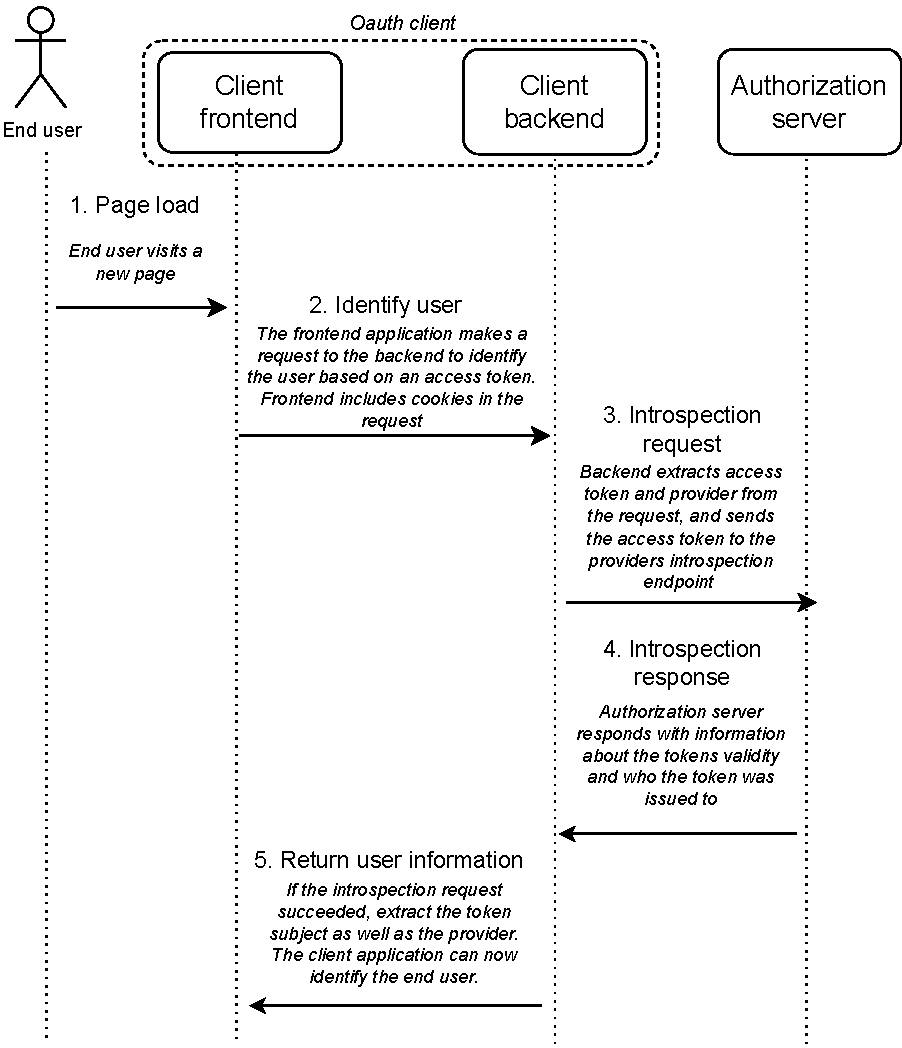
\includegraphics[height=165mm]{assets/introspection_client_flow.drawio.pdf}
	\caption{Network traffic of the access token introspection}
	\label{introspection_client_flow}
\end{figure}

\subsubsection{Refreshing access tokens}
Since access tokens are only valid for a specific time, it is useful to be able to refresh existing tokens, ideally without requiring user input.
To achieve this, OAuth clients can request refresh tokens, which can be used to request new access tokens.
While they do improve the user experience, refresh tokens weaken the security of the system, as their long expiry time increases the probability that they will be leaked.

In the client example, a refresh token is requested by setting the $access\_type$ to offline in the authorization code request (step 3 in figure \ref{client_auth_requests}).
The refresh token is then stored as a cookie in the end user's browser, similarly to the access token.
The refresh token can now be used when the client frontend interacts with the backend.
In the client example, the refresh token is used in combination with the token introspection request.
If a refresh token is set and the access token is not set, or if the introspection response fails (step 4 in figure \ref{introspection_client_flow}), the backend server will attempt to request a new access token based on the stored refresh token.
If the refresh succeeds, the client stores the updated access token and retries the earlier token introspection.
If the refresh fails, the refresh token and access token are removed.

\subsection{Token storage}
\label{sec:implementation-storage}
As described in section \ref{sec:background-storage}, a number of options exist for storing data in web browsers.
The most secure storage solution for an OAuth client would be to temporarily store tokens in JavaScript, with closures providing some additional security.
Such a solution would not however provide any persistence, and as such the end user would have to authenticate every time they start a new browser session.
To improve the user experience, the example client persists the access tokens, allowing users to stay logged in across multiple sessions.
When choosing to persist data developers have two practical options: the web storage API and cookies.
Due to its vulnerability to XSS attacks, the web storage API is not an optimal solution for storing sensitive information.
We instead opt for cookies to store any client-specific information when obtaining an access token, described in section \ref{sec:implementation:access-token}.

Many cookie flags that improve the storage security, described in section \ref{sec:background-storage}, are essential when storing sensitive data such as access tokens.
The cookies are marked as \textit{HttpOnly}, causing the cookies to be included in requests while keeping them completely inaccessible for the frontend application.
Instead, only the backend application can set and modify the cookies.
Any sensitive cookies should also be marked as \textit{Secure}, causing them to only be included in HTTPS requests.
This is a critical flag to include, as any network attacker could intercept sensitive cookies in transit if they are included in regular HTTP traffic.
Cookies should also have an appropriate \textit{SameSite} value.
The state, code verifier and provider should be stored with the \textit{Lax} SameSite policy, as they are accessed in a request that is initiated from the authorization server.
The access token and refresh token should instead be stored with the \textit{Strict} policy, as it does not need to be included in requests with any external origin.

To further limit the possibility of sensitive tokens leaking, tokens can be encrypted before storage.
Since all communication with the authorization server in an OAuth client with a separate frontend and backend flows through the backend server, the end user does not need access to the original, unencrypted access token, code verifier or OAuth provider.
If all the values stored in the client are encrypted, an attacker is unable to steal the original tokens.
The provided security benefit from this is however quite limited, as the client backend will accept and decrypt any token, without any way to verify if it was stolen or not.
Instead, the encrypted cookies have a greater impact on the authorization code flow, as modifying the temporarily stored state, code verifier or OAuth provider is more difficult.
An attacker is required to interact with the backend client themselves to obtain modified values that are encrypted with the correct key, allowing the client to limit what type of values are generated.
This also makes it easier to investigate malicious activity, since the attacker has to interact with the legitimate client to pull off any attack.
\subsection{Proof Key for Code Exchange}
\label{sec:pkce}
To protect against authorization code injection, the OAuth 2.0 Security Best Current Practice \citep{ietf-oauth-security-topics-27} recommends using Proof Key for Code Exchange (PKCE) to bind authorization codes to client instances \citep{rfc7636}.

PKCE relies on creating a code verifier in the initial authorization code request (step 2 in figure \ref{client_auth_requests}).
The code verifier should be a random string with between 43 and 128 characters.
This code verifier should be temporarily stored by the client.
In our example client, the value is stored as a cookie in the user's browser.
After generating the code verifier, the client generates a code challenge by hashing the code verifier.
The code challenge should be generated using the SHA256 algorithm \citep{dang_secure_2015} if possible.
The generated code challenge is sent to the authorization server together with the code request.
The used code challenge method, such as \textit{S256} if SHA256 is used, is also included in the request.

After receiving the authorization code, the OAuth client requests an access token from the authorization server (step 6 in figure \ref{client_auth_requests}).
The original code verifier is included in the access token request.
The authorization server computes a code challenge based on the verifier and the previously sent challenge method and compares it with the initial code challenge.
If the two code challenge values do not match, the authorization server interrupts the access token generation.




\subsection{Explicit user intention tracking}
To protect against CSRF attacks and IdP mix-up attacks, described in sections \ref{sec:vulnerabilities-state} and \ref{sec:vulnerabilities-idp}, additional controls should be used to keep track of user actions.
To alleviate these issues, the authorization code flow described in figure \ref{client_auth_requests} contains some additional checks that are not mandatory in the OAuth 2.0 authorization code flow described in figure \ref{oauth_code_flow}.
The chosen provider is tracked in each step, with separate routes for separate providers to limit the chance for a mix-up.
Additionally, the original chosen provider is stored as a cookie, allowing the client to validate that the actual used provider is the same as the provider chosen by the user.

Step 5 of figure \ref{client_auth_requests}  is also added as an extra guard against CSRF and IdP mix-up attacks.
The redirect via the frontend prompting for user consent is not required to request an access token, which could be handled completely in the backend.
It is however useful as a prompt for the user to confirm that they intend to sign in to the page, and that they chose to sign in with a specific provider.
If the step was missing, it is possible that an attacker could craft a CSRF request that signs in the user as the attacker, or that signs in the user using the wrong authorization server.
